%************************************************
\chapter[Background]{Background}\label{ch:Background}
%************************************************

\begin{flushright}{\slshape Nicholas of Morimondo: ``We no longer have the learning of the ancients, the age of giants is past!'' \\
William of Baskerville: ``We are dwarfs, but dwarfs who stand on the shoulders of those giants, and small though we are, we sometimes manage to see farther on the horizon than they.''} \\ \medskip
    ---  The Name of the Rose, Umberto Eco
\end{flushright}

Since the beginning of this work, the aim was always to avoid ``reinventing the wheel''. By doing our initial analysis of the state of the art in robotic software development, software engineering, embedded system, modelling languages and formal methods, we realised that most of the necessary tooling was already available. The effort was in combining the existing technology to produce a result that is greater than the parts. Our target was to enhance robot software development by integrating methods, techniques and technologies from other fields.

This section provides to the reader all the necessary background to understand the technologies and the tools that will be used in this work. First, we present the Robot Operating System by giving an overview of its main elements, functionalities and structure. Then we move to modelling languages. The first one is the Architecture Analysis and Design Language (AADL), the main modelling language that we will use to design and describe robot architectures. We present the main components and their significance to our work. Moreover, we provide graphical and textual examples on how to represent basic AADL elements. 
%To conclude, we give a brief description of the two data modelling languages used in this work: Abstract Syntax Notation One and JSON in combination with JSON schema.

\newpage

\minitoc
\newpage

\begin{figure}[t]
    \centering
    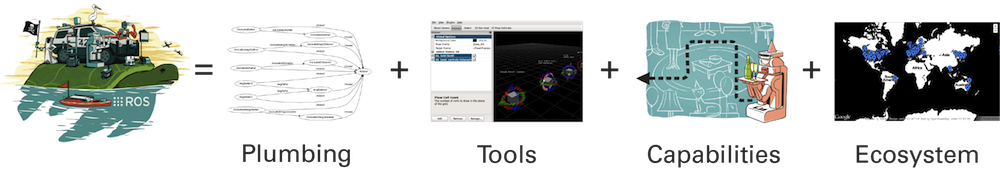
\includegraphics[width=0.95\textwidth]{gfx/ros/ros_equation}
    \caption{The ``ROS Equation''. It shows the key element composing the ROS environment. }\label{fig:ros}
\end{figure}

\section{Robot Operating System}
\label{sec:ros}
The Robot Operating System, as the name suggests, is an open source, meta-operating system (or middleware) designed to develop robot software. By creating a meta level on top of the operating system, ROS provides a series of functionalities to implement its distributed architecture, including  hardware abstraction, low-level device control, implementation of commonly-used functionality, message-passing between processes, and package management. It also provides tools and libraries for obtaining, building, writing, and running software across multiple platforms.

The main goal of ROS is to support code reuse in robotic. This is achieved by following the philosophy of giving great freedom to the developers and support them by providing a robust and flexible communication architecture, by developing a collection of tools and by creating a thriving community. Figure~\ref{fig:ros} perfectly synthesize what ROS is, it is not a framework, it does not provide libraries, guidelines, or developing rules. ROS is a communication infrastructure, a distributed network of processes to be individually designed and loosely coupled at runtime. A set of tools, ROS provides multiple interfaces to inspect (\eg, \texttt{rviz}, \texttt{rqt\_graph}) the system, log (\eg, \texttt{rosbag}) the output, organise (\eg, \texttt{roslaunch}) the components, visualise (\eg, \texttt{rqt\_plot}, \texttt{image\_view}) data streams, navigate (\eg, \texttt{rospack}, \texttt{roscd}) the file system, build (\eg, \texttt{catkin}) the environment, and more. A repository of already available software modules implementing functionalities from low-level device drivers, to high-level planning, navigation, or manipulation algorithms. Lastly, ROS is the engaging community created thousand of developer around all world working toghether to develop ROS packages and sharing them using the ROS Wiki\footnote{http://wiki.ros.org/} and supporting each other through ROS Question \& Answers\footnote{https://answers.ros.org/questions/}.

\begin{figure}[t]
    \centering
    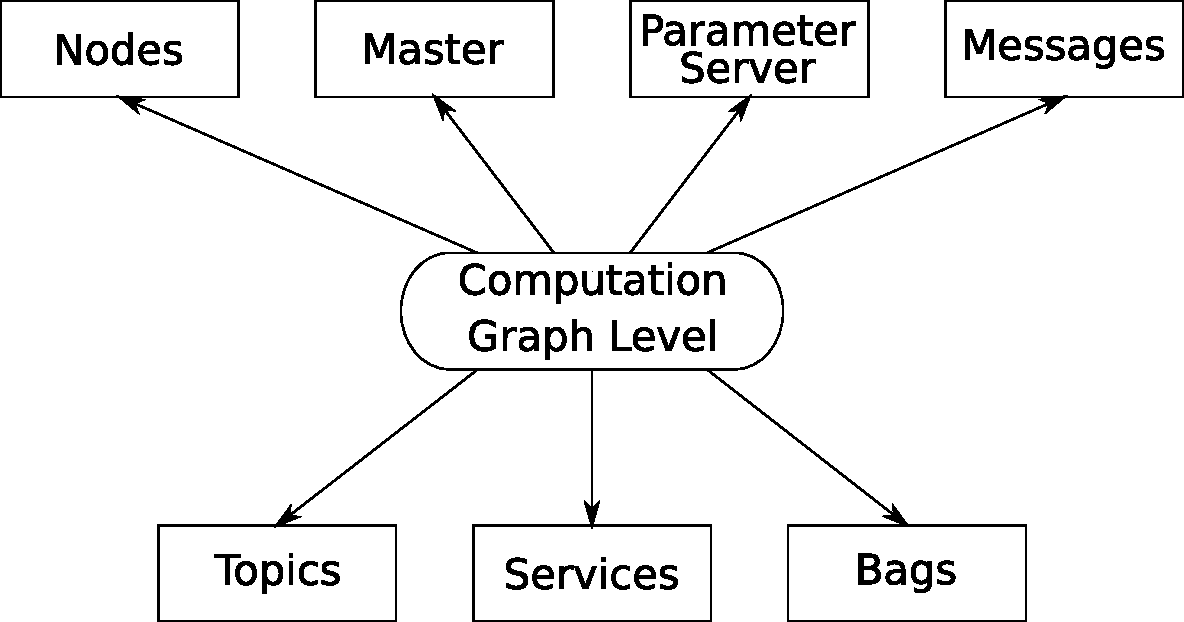
\includegraphics[width=0.8\textwidth]{gfx/ros/graph}
    \caption{The ROS Computation Graph.}\label{fig:ros-graph}
\end{figure}

\subsection{Computation graph}
Central to the structure of ROS is the Computation Graph (Figure~\ref{fig:ros-graph}), it represents the abstract infrastructure connecting all the elements of the ROS middleware. It should not be confused with the runtime graph composed by the currently active elements of a ROS architecture, which is just one of the possible instances.  The Computation Graph consists in a peer-to-peer network where all the hypothetical ROS applications can connect to process, share, and exchange data, it defines the backbone of any ROS-based architecture. The main conceptual components connected to the abstract Computation Graph are nodes, as data generators and processors, the Master, as coordinator and name server, the Parameter Server, as parameter centraliser and provider, messages, as main form of data exchange, services and topics, as the prime communication channels, and bags, as pure data consumer.

\begin{itemize}
\item Nodes. They processes that perform computation, they produce, process and consume the data circulated in the graph. The modular design of ROS is based on the fine-grained functionalities implemented by the nodes. Each of them is in charge of a specific subsystem of the robot (\eg, a sensor, an actuator, localisation, planning, \etc). 
\item Master. The role of the master is to provide a name registration service and a lookup system to the rest of the Computation Graph. It mediates the communication between nodes by initiating the connection between them. 
\item Parameter Server. ROS provides a centralised location to store all the parameters of the nodes. Parameters can be global (\eg, \texttt{/use\_sim\_time}) or defined in the namespace of a node (\eg, \texttt{/talker/frequency}).
\item Messages. They can appear in various forms depending on the specific protocol used, however, all the communication in ROS happens trough the exchange of messages. A message is simply a data structure, comprising typed fields (\eg, integer, floating point, boolean, \etc). Messages can include arbitrarily nested structures and arrays.
\item Topics. They represent the asynchronous communication system implemented by ROS based on the publish/subscribe paradigm. Topics are named channel, and nodes can subscribe to them to receive messages, or publish on them to produce messages.
\item Services. They implements the ROS version of a synchronous communication system based on the client/server paradigm. Differently from topics, they are not a named channel, but remote functionalities identified by a name. Communication happens through an exchange of two messages: a request and a response.
\item Bags. Bags are a format for saving and playing back ROS message data. Bags are an important mechanism for storing data, such as sensor data, that can be difficult to collect but is necessary for developing and testing algorithms. 
\end{itemize}

Each ROS architecture represent a runtime instantiation of the Computation Graph where vertexes are represented by nodes and the other active elements (\ie, Master, Parameter server and, if active, the bag recording system), and edges are represented by communication systems (\ie, service and topics). The existence of messages in the runtime version of the Computation Graph is transient, since they are generated, exchanged and then consumed. However, when they exist, they form a temporary ternary relation with the node and the communication channel.

While the Master acts as a coordinator to initiate the communication between nodes, after it is established they are connected to each others directly. For example, nodes that subscribe to a topic will request connections from nodes that publish that topic, and will establish that connection over an agreed upon connection protocol. The most common protocol used in a ROS is called TCPROS, which uses standard TCP/IP sockets. This architecture allows for decoupled operation, where the names are the primary means by which larger and more complex systems can be built. Names have a very important role in ROS: nodes, topics, services, and parameters all have names. Every ROS client library supports command-line remapping of names, which means a compiled program can be reconfigured at runtime to operate in a different Computation Graph topology.

For example, to read the measurements produced by a Hokuyo laser range-finder, it is possible to use the \textit{hokuyo\_node} driver, which interfaces with the hardware component and publishes \textit{LaserScan} messages on the \texttt{/scan} topic. To process that data, a developer might implement a \textit{laser\_manager} node that subscribes to messages on the \texttt{/scan} topic. After subscription, the new node would automatically start receiving messages from the laser. The two sides are completely decoupled. All \textit{hokuyo\_node} does is publish laser range-finder measurements, without knowledge of which node will consume the messages. The only thing \textit{laser\_ma\-na\-ger} has to do is subscribe to \texttt{/scan}, without knowledge of whether the topic is active or which node is generating the messages. The two nodes can be started, closed, and restarted, in any order, without inducing any error conditions. Later, it may be necessary to add a second laser range-finder to the robot, this requires to reconfigure the architecture. This can be done easily by remapping the names of nodes and topics. Two instances of the \textit{hokuyo\_node} are now necessary, and each of them can have its own name to coexist in the graph as two different vertexes. Moreover, since they provide two different measurement, each \texttt{/scan} topic can be renamed accordingly (\eg, \texttt{/left/scan} and \texttt{/right/scan}). For the \textit{laser\_manager} to reach one of the topic, it is possible to follow the same remapping procedure, where the \texttt{/scan} topic is renamed to match the output of the driver.

\begin{figure}[t]
    \centering
    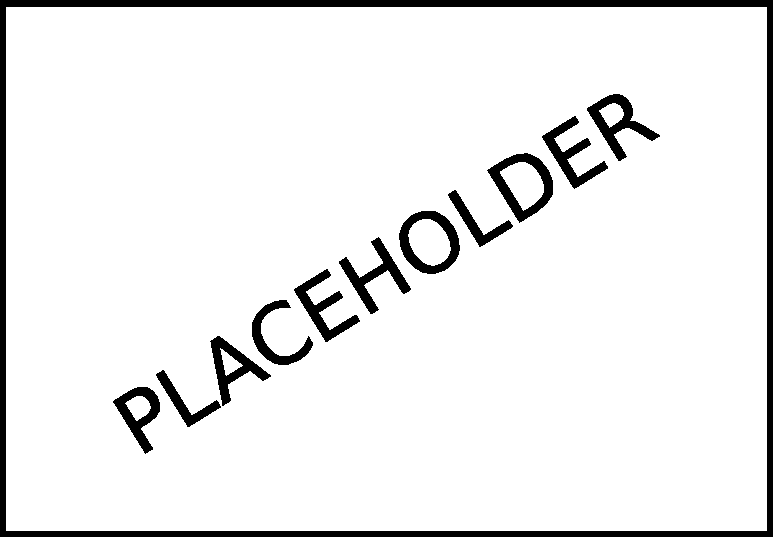
\includegraphics[width=0.8\textwidth]{gfx/placeholder}
    \caption{TODO}\label{fig:ros-master}
\end{figure}

\subsection{Components}
In the Computation Graph the main active elements (\ie, performing computations) are nodes, they implements directly the functionalities of the robot and appears in the graph as a multitude of instances. However, other actors exists that perform small, yet crucial roles in the correct execution of a ROS architecture. The Master as communication mediator, the Parameter server to configure the nodes and the environment, and, even though it is not in the main concept of the Computation Graph, the Transformation Frame, a centralised system handling coordinate transformations in the robot.

\paragraph{Master} It exists as a single instance in the runtime graph, and it must be run before every other element of the architecture using the command \texttt{roscore}. This is necessary because the Master acts as a name service, when a node is started it is registered to the Master, the same happens every time a new topic, both as a subscriber or publisher, or a new service, both as client and server,  is created. By communicating with the Master, nodes can receive information about other registered nodes and their advertised topics and service, and, eventually, create the necessary point-to-point connections.

The communication between the Master and the nodes happens using a XML Remote Procedure Call (XMLRPC) protocol, which is an HTTP-based protocol that does not maintain an active connections. Nodes interact with the Master when they need to register a new communication or when they need to retrieve registration information. The Master will also make callbacks to these nodes when this registration information changes, which allows nodes to dynamically create connections as new nodes are run. The non-permanent connection combined with the lightweight XMLRPC protocol make it possible for the Master to manage  very large and complex environments.

Figure~\ref{fig:ros-master} shows an example on how the Master mediates the connection between two nodes. At the beginning there are two independent nodes. A typical sequence of events starts with the \textit{camera} node notifying the Master that it wants to publish \textit{Image} messages on the topic \texttt{/images}. The combination of node and topic is registered in the Master, but since there is no subscriber yet, no data is actually sent. At some point, without any knowledge about the existing nodes or topics, the \textit{image\_viewer} node register in the Master a subscriber for the topic \texttt{/images}. Since the topic has now both a subscriber and a publisher, the Master can notify the two nodes, so they can establish a direct connection and exchange messages. From this point the Master is not involved in the communication any more, until one of the two nodes shuts down and its topic information is unregistered.

\paragraph{Parameter Server}  As for the Master, only one instance of the Parameter Server exists in the system. This is not the only trait they share, since both are started together with the \texttt{roscore} command. The Parameter server is a shared, multi-variate dictionary that is accessible via network APIs. Nodes use this server to store and retrieve parameters at runtime. As it is not designed for high-performance, it is best used for static, non-binary data such as configuration parameters. It is meant to be globally viewable so that tools can easily inspect the configuration state of the system and modify if necessary.

As mentioned before, names have an important role in defining a ROS architecture. The Parameter server follows the same convention used when naming topics and nodes. This means that ROS parameters have a hierarchy based on the namespace introduced by the other elements of the graph. In practice, parameters can be accessed globally when using the full definition of their names (\eg, \texttt{/camera/right/exposure}), while are resolved depending on the current namespace when using a partial name (\eg, \texttt{right/exposure}). The hierarchical scheme also allows parameters to be accessed individually or as a tree. For example, let us consider a system where two parameters are exposed in the same namespace: \texttt{/camera/left/exposure} and \texttt{/camera/left/resolution}. It is possible to access each parameter directly and get their individual values or use a reference to the namespace (\ie, \texttt{/camera/left}) to receive a dictionary containing all the parameters existing in that namespace.

\paragraph{Nodes} They are the main executable element active in the graph. Multiple different nodes and multiple instances of the same node can be running at any time. They represent the variability of the system, since their implementation and topology is defined by the developer. The aim of the nodes is to implement fine-grained functionalities of the robot, for example they can implement a single device driver, or a velocity controller, encapsulate a planning algorithm, or a localization system. ROS gives absolute freedom to the developer in the design and implementation of the nodes, however, to interact with the Computation Graph, few standard interfaces are defined.

To interact with topics, nodes implements publishers and subscribers. A publisher needs to be registered on a specific topic, and then can be called at any point during execution to generate a specific message and circulate it in the graph. Subscribers reference a topic and are bound to a function as a callback. When a new messages is detected on the topic, the callback is executed providing the instance of the message as parameter. Interaction with services is similar, it happens using clients and servers. To advertise a service a node needs to implement a server and bind it to a callback. The callback is triggered by a request message, and it is expected to return a response message with the result of the computation. To use a service a nodes implements a client. After binding it to the correct service, the client can be invoked at any time. While the remote service is in execution, the client node is locked waiting for the completion. A similar approach (\ie, client and server) is used for action, with the significant different that the execution is non-blocking.

There is only one thing a process needs to do to be part of the runtime graph and be considered a node: register itself to the Master. This single requirement encompasses the philosophy of ROS of giving basically no restriction to the developer. While not required, there is another element that characterise a ROS node: the spinner. The ROS spinner is the main loop of the component, it polls all subscribers, publishers, clients, servers to detect any new message or request. ROS provides few option when implementing it.
\begin{itemize}
\item \textit{single spin}. The developer controls the frequency of the polling by invoking the spin command when necessary. It is useful when implementing a task that has to be repeated periodically (\eg, fixed frequency multiplexer).
\item \textit{single-thread spin}.The main execution thread of the process is locked in the polling activity, until a new messages is received by a subscriber or a server. This approach is used when the action of the node are purely reactive (\eg, a control component waiting for set-points).
\item \textit{multi-thread spin}. As before, the process is locked when the spinner is active, but instead of sequentially switching the execution between the polling activity and the callbacks, multiple threads are used, providing a variable level of parallelisation. This approach has to be used when the node implements long callback with a fixed frequency (\eg, low-level sensor driver).
\item \textit{asynchronous spinner}. This is an alternative implementation of a multi-thread spinner. In this case the polling activity is not blocking, since it is implemented in a separate thread, and each callback is managed in a new thread. When implementing an asynchronous spinner, the developer has to be aware of all the potential concurrency problems introduced. Asynchronous implementations are useful when the node has to implement fixed-frequency callbacks while maintaining control on the main thread (\eg, sensor driver with independent communication threads).
\end{itemize}

The decentralised processing architecture implemented by ROS nodes provides several benefits to the overall system. There is additional fault tolerance, since an unexpected shutdown of a node may compromise the functionality of a subsystem, but not of the entire robot. With respect to a monolithic system, code complexity is significantly reduced, since the implementation is distributed in the single node and all the coordination and communication activities are managed by the Computation Graph architecture. Implementation details are also well hidden as the nodes expose a minimal API to the rest of the graph and alternate implementations, even in other programming languages, can easily be substituted.

ROS is designed to be a meta-operating system, and its focus is on accessibility, component reuse and hardware abstraction. Therefore, differently from other robotic frameworks, it does not provide a predefined structure for nodes and it leaves freedom to the developer when implementing them. The ROS-specific functionalities, publish and subscribe to topics, invoke and offer services, access the Parameter server, are all provided by a thin implementation layer called ROS Client Library. It is a collection of implementations, libraries and APIs that assist the developer in developing ROS nodes. Perfectly in line with the flexibility promoted by ROS, such libraries can be implemented in any programming language, since they need to implement general protocols like XMLRPC and TCPROS (\ie, ROS transport layer based on TCP/IP). Currently, there are three main client libraries, with a particular focus on C++ and Python.
\begin{itemize}
\item \textit{roscpp}.The C++ implementation of the ROS Client Library. Given the language of choice, this library is designed for efficiency, high execution speed and robustness. It is the most widely used library and it should be used when targeting the final deployment of a ROS-based architecture. 
\item \textit{rospy}. This is the version of the ROS Client Library implemented in Python. It is aimed at providing advantages of an object-oriented scripting language, namely reduce development time and provide implementation flexibility to promote rapid prototyping and testing. Moreover, it is  ideal for non-critical-path code, such as configuration and initialization code
\item \textit{roslisp}. While actively supported, this implementation of the ROS Client Library in LISP exists mostly for legacy reasons. It is used for the development of the planning libraries. 
\end{itemize}

\begin{figure}[t]
    \centering
    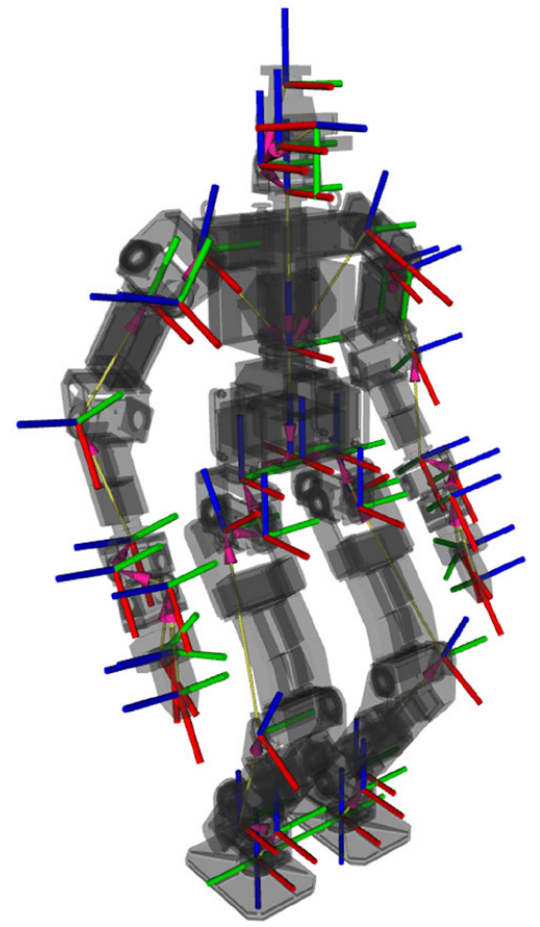
\includegraphics[width=0.5\textwidth]{gfx/ros/tf_frames}
    \caption{A graphical representation of all the coordinate frames necessary to completely describe the structure of the THORMANG3}\label{fig:ros-tf}
\end{figure}

\paragraph{Transformation frames} When describing the physical structure of a robot, the position of each element has to be defined with respect to the others. For example, to estimate the position of a mobile robot though vision, it is necessary to know where the camera is located on the robot, to estimate then the expected position of some reference points and translate it back to the base of the robot. The more degrees of mobility a robot has the more complex this description become, Figure~\ref{fig:ros-tf} shows all the possible coordinate frame in a THORMANG3 robot. Each joint of the robot can move with respect to the previous one, therefore every point on the robot and in space can be defined with respect to a multitude of coordinates system, since each of these systems defines a new rigid transformation. The complexity of managing all the coordinate systems grows dramatically every time a new one is defined, and the number of total frame may increase dynamically during execution, since any new interactive element in the environment (\eg, an obstacle to avoid or an object to grasp)  may create a new one. Given how central coordinate frames are when developing a robot, ROS provides its own set of tools to manage them: \textit{transformation frames}, commonly referred as \textit{tf}.

\begin{figure}[t]
    \centering
    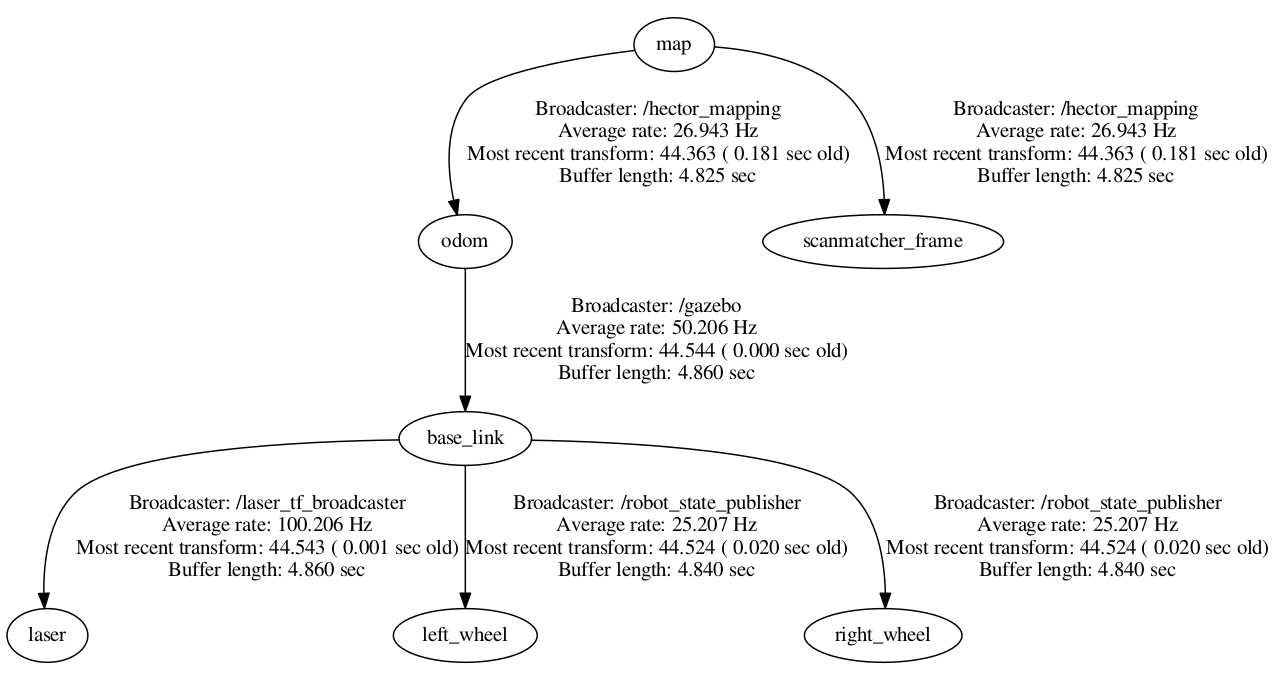
\includegraphics[width=0.95\textwidth]{gfx/ros/tf_tree}
    \caption{An example of a complete \textit{tf} tree for a mobile robot.}\label{fig:ros-tf-tree}
\end{figure}

Of course, \textit{tf} cannot replace the designer in defining the correct reference frames for each element of the robot. However, what it does is to create a distributed system to manage coordinates that free the developer from worrying about conversions between one and another. Thanks to \textit{tf}, at any moment in time, the developer can define a location in space in a specific coordinate system and easily convert it in a different one. To achieve this, it is necessary to maintain a consistent transformation tree, an example is shown in Figure~\ref{fig:ros-tf-tree}. \textit{tf} provides conversion from any frame to another (\eg, from \texttt{map} to \texttt{right\_wheel}) at any point in time, but only if a complete chain of transformation between the two frames exist in the correct time frame.

To maintain ha consistent transformation tree, the developer can use the many accessory tools provided. When a coordinate system does not move with respect to its parent reference frame (\eg, the position of a sensor on a robot), it is considered a static transform. They can be broadcast using the \textit{static\_transform\_publisher} node, which can be configured to create a latched publisher that provides an up to date static transform every time is requested. A transform is dynamic when it changes its relative position in time (\eg, the position of the robot with respect to the map). In this case, to update the transformation tree, it is necessary to use the APIs provided by \textit{tf} during the execution of the node responsible of estimating the dynamic transform. The node has to declare a \textit{tf} broadcaster, then, at any time during the execution, can be used to notify the updated version of the dynamic transform to the system.  Since \textit{tf} can estimate the chain of transformations at any point in the past, it is important that each new dynamic transform is broadcast with the correct timestamp.

When a node needs to query \textit{tf} to request a specific transform, it can do that by declaring a \textit{tf} listener. The listener can be used to receive any kind of coordinate frame at any point in time, by specifying during the invocation a parent frame, a child frame and a timestamp. While there is no central location containing all the coordinate systems, and \textit{tf} uses a distributed architecture to store and share them, most of the actual computation happens in a ``transformations buffer'' embedded inside the listener. This means that while, theoretically, it is possible for \textit{tf} to unravel the entire history of a coordinate system, in practice this is limited by the buffer created by the specific listener. However, present-time transform are always available at any depth of the transformation tree. In summary, \textit{tf} is one of the most powerful tool provided by ROS, since it removes a significant burden to the developer when designing and implementing complex interconnected robotic systems.

\paragraph{Launch files} The Master, together with the Parameter server, are run by the \texttt{roscore} command, nodes are activated using the \texttt{rosrun} command and \textit{tf} provides a special command to broadcast static transforms. When an architecture grows, so does the complexity of executing all its elements in the correct order and with the right configuration. In order to alleviate this burden ROS provides a system called \texttt{roslaunch}.

A launch file processed by \texttt{roslaunch} is an XML file containing a list of the elements that needs to be run for a specific architecture. The Master and the Parameter server are run automatically when executing the \texttt{roslaunch}, hence by writing a complete enough launch file it is possible to execute the entire architecture with a single command.

A launch file is highly configurable. Using the XML tags, a developer can: rename nodes, remap topics, provide command line configuration, include complete parameter profiles through YAML files, define global parameters, enable node restart and include other launch files. The potentially hierarchical structure of launch files can be used to obtain a partial description of the runtime topology of the architecture, however, currently there is not tool in ROS to provide this kind of visualisation.

\subsection{Communication}
As any graph, the ROS runtime graph is composed by vertices and edges. In the previous section, we discussed the main processing elements, the vertices, while in this section we cover all the communication protocols, the edges. One of the main characteristics of ROS is its distributed architecture, nodes can be executed on different machines, but the complexity of transmitting messages through multiple physical mediums is hidden by the middleware functionalities. Communication in ROS happens mostly through a very flexible protocol based on a publish/subscribe approach: the topics. While this one-size-fits-all approach works for most situation, ROS also provides alternative solutions like services and actions.

\paragraph{Message} Central to the communication system of ROS is the concept of messages, since they are used, in different forms, by all protocols. Nodes communicating through topics exchange messages directly, the client/server interaction implemented by services is achieved by a pair of messages, while actions use a more complex system that relies on a triple of explicit messages combined with hidden messages used by the protocol.

In every aspect of its design, ROS promotes simplicity, thin approaches and a straightforward implementation, messages are no exception. They are simple data structure, composed by constants or typed fields. The field types can be:
\begin{itemize}
\item one of the standard built-in types. They are the common types usually found in programming languages. The available types are: boolean, a logic value that can be \textit{true} or \textit{false}, integer, there are signed and unsigned options with different sizes (\ie, 8-bit, 16-bit, 32-bit or 64-bit), floating point, for any non-integer number, available as 32-bit and 64-bit, string, any ASCII string, therefore Unicode characters are not supported, time and duration, represented as a pair of seconds and nanoseconds;
\item other messages. ROS supports a nested structure for message typing, this means that any other message type, pre-defined in ROS or custom-defined by the developer, can be used as a type in field in a message. This promotes reuse of standard, and previously defined, messages, and a hierarchy of concepts. For example, it is natural to assume that a \textit{Polygon} is defined as a list of \textit{Point}, or that a \textit{Pose} is composed by \textit{Position} and \textit{Orientation};
\item any of the previous type can be arranged in a fixed-length array or in a dynamic list. Together with the nested structure, it makes the design of ROS message simple yet powerful;
\item the special \textit{Header} type. While it is defined as a message in the package \textit{std\_msgs}, the \textit{Header} is unique since it can be referred directly without specifying the package and it is meant to exists as an unique field on the root of the message to provide a generalised ID. The \textit{Header} type has three fields: \texttt{seq}, an unsigned long integer designed to be an increasing identifier of the message instance, \texttt{stamp}, the timestamp of the creation of the message, and \texttt{frame\_id}, a string containing the name of the frame of reference associated with the message.
\end{itemize}

Messages are defined using a very simple message definition language. Each field is described by a pair of keywords, one defining the type and the other defining the name. To define an array or a list, it is possible to add two square brackets near the type, eventually specifying the size (\eg, \texttt{int32[]} or \texttt{Point[3]}). Constants are defined in the same way as fields, except that it also assigns a value using the equal sign (\ie, \texttt{=}). No other data structure is allowed in the message definition, to nest type it is necessary to define them in a different message and include them as types. Multi-part messages used in services and actions are defined following the same rules, each part is separated by the others using ``\texttt{-{}-{}-}'' as a separator.

\paragraph{Topic} The main communication system of ROS is based on an asynchronous protocol implementing an anonymous publish/subscribe paradigm. In practise, topics are named buses that nodes can use to exchange messages. Given the publish/subscribe paradigm, combined with the anonymity of the message-based communication, the use of topics decouples the production of information from its consumption. Without any explicit information in the content of the message, nodes are not aware of who they are communicating with. Instead, nodes that are interested in a specific data stream subscribe to the relevant topic, while nodes that generate data publish to the relevant topic. A for many other design choices, ROS is very flexible and permissive in the structure of topics, hence, multiple publisher and multiple subscribers can read and write from the same topic at the same time.

Topics are intended for unidirectional, streaming communication, therefore, they are not supposed to provide a reliable communication. Topics do not guarantee the delivery of the messages nor have an expected delivery time. While the communication is mostly reliable when the two connected nodes are executed on the same machine, the potentially distributed nature of a ROS architecture (\ie, nodes running on different machines) combined with the unknown physical communication medium force the developer to treat ROS topics as a communication channel subject to potential data loss.

While there is no limit on the number of publishers and subscribers connected to a topic, they all need to write or expect the same message. Topics are strongly typed by the ROS message type used to publish to them, and nodes can only receive messages with a matching type. The Master does not enforce type consistency among the publishers, however new publisher with a mismatched type faces a communication error when trying to write on the topic. On the contrary, the Master will block subscribers from establish message transport if the types do not match. Lastly, all ROS clients implements a client-side check to make sure that an MD5 computed from the message file matches the signature of the topic. This check ensures nodes are compiled from a consistent code base.

To implement topic communication, ROS currently supports message transport based on both TCP and UDP. The TCP/IP is the default transport, known as TCPROS, and streams message data over persistent TCP/IP connections. Since it is the default, TCPROS is also the only transport that ROS Client libraries are required to support. The UDP transport, which is known as UDPROS, is currently supported only by the C++ ROS Client Library (\ie, \textit{roscpp}). UDPROS is a low-latency, lossy transport, hence is best suited for non-critical tasks requiring high-speed communication and faster response (\eg, teleoperation). ROS nodes negotiate the desired transport at runtime, therefore, a node implemented to use the UDPROS transport can always fallback on TCPROS if the destination node does not support it. This negotiation model enables new transports to be added over time as compelling use cases arise. 

\paragraph{Service} The publish/subscribe communication provided by topics is extremely flexible and suitable for a variety of situations in a robotic architecture. However, its \textit{n-to-n}, one-way, asynchronous transport, combined by the implicit unreliability of the communication, is not appropriate for all interactions. In distributed systems it is often necessary to implement synchronous, bi-directional, reliable interactions, in ROS this is achieved using services. They implement a remote procedure call (RPC) based on a client/server paradigm. Services are defined by a pair of messages: one for the request sent by the client, and one for the reply sent by the server. Differently from topics, the name of the service advertised by a node does not represent the communication channel, but an entry on the Master. In practices, it means that differently from a topic, it is not possible for an external entity to ``listen'' to a service communication.

Service calls are one-shot interactions. A client start the communication by requesting to the Master who is exposing a specific service. After that it establish a direct connection with the server and send the request message, after the service-specific processing, the server sends back the appropriate response and the connection is closed. Multiple server can expose the same service (\ie, advertise a service with the same name), there is no way for the client to pick a specific server, and the Master will provide one of all the available. In extreme cases, this means that successive calls of the same service will be answered by different servers. To avoid this, a client can make a persistent connection to a service, which enables higher performance at the cost of less robustness to service provider changes.

As for topics, services are strongly typed by the service message they use. In this case is the server that imposes the type of the communication, since it is the one exposing the service. Clients are not allowed to establish a communication if the requested type does not match the server. As an extra layer of consistency, services are versioned by an MD5 sum of the service message file. Nodes, both implementing server and client, are only allowed to start a service interaction if the the MD5 sum matches.

\begin{figure}[t]
    \centering
    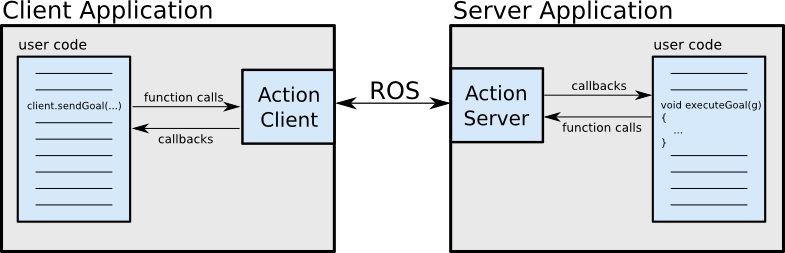
\includegraphics[width=0.95\textwidth]{gfx/ros/action}
    \caption{Communication interface of the ROS \textit{actionlib}.}\label{fig:ros-action}
\end{figure}

\paragraph{Action} Services implement a synchronous client/server protocol, this means that after sending the request, the client needs to wait until the server provides the response. This approach is suitable for short interactions, when the waiting time is not detrimental to the correct execution of the client, however, it is incompatible with requests that trigger long multi-step procedures. The ROS answer to an asynchronous client/server protocol is the \textit{actionlib} package, or ``actions''.

Actions realises their asynchronous protocol by using a collection of topics, this ``under the hood'' implementation is hidden to nodes by providing two interfaces: an \textit{ActionClient} and an \textit{ActionServer}. The client and server then provide a simple API for developer to request goals (on the client side) or to execute goals (on the server side) via function calls and callbacks. Since action are designed to trigger complex and long activities, they implement a system to track the evolution and the current status of any active task, and to interrupt or pause any active action.

As said before, the actual communication is implemented through topics, to fulfil all the expected functionalities, the action protocol uses five different communication channels. Two of them are from the client to the server: goal, used to activate the action and send the current goal, and cancel, used to interrupt an active action. The remaining three are from the server to the client: status, used to notify clients on the current state of a goal (\eg, active or paused), feedback, used to send periodic auxiliary information about a task, result, used to send to the client a one-time information upon completion of a goal.

While not all topics are used directly, to implement the action protocol, the developer needs to define an action message file. The file is composed by three different parts, each one representing a different phase of the protocol: activate the action, receive updates and receive the result. 
\begin{itemize}
\item Goal: this field represent the final goal of the task and it is used to activate the action. It is the asynchronous counterpart of the service request, and as for the request it is sent by the \textit{ActionClient} to the \textit{ActionServer}. For instance, for a complex navigation task, the goal would a \textit{PoseStamped} message containing the destination of the robot.
\item Feedback: this field provides incremental updates on the current status of the goal. It is unique to the action protocol and it has no counterpart in a service. This message is periodically sent by the server to the client. In the case of the navigation task, a feedback message would be the current position of the robot along the path.
\item Result: this field return the result of the task and represent the end of the action. Its synchronous counterpart is the service response provided by the server. A result message is sent only once by \textit{ActionServer} to the \textit{ActionClient} upon completion of the goal. In the example of a complex navigation task the result is not particularly meaningful, however, it is significant, for instance, when the task of the action is to calculate a complex behaviour for the robot. In this case, the result message contains the resulting behaviour.
\end{itemize}

\subsection{Filesystem}
Given its nature as a middleware and meta-operating system, additionally to all the communication and execution functionalities, ROS also provides a filesystem on top of the original provided by the native OS. It is possible to navigate this ROS filesystem using a series of commands, for instance, \texttt{roscd} to move to a specific folder, or \texttt{rospack depends} to list all the dependencies of a specific component, and many more.

Central to the design of the ROS filesystem is the concept of packages. A package might contain nodes, a ROS-independent library, a dataset, configuration files, a third-party software, or anything that can be logically considered part of a module. The goal of these packages is to provide useful functionalities in an easy-to-consume manner, to promote software re-usability. In general, ROS packages follow a "Goldilocks" principle: enough content to be functionally complete, but without overloading the package which become heavyweight and difficult to manage.

The build process of ROS is atomic with respect of packages, this means, for instance, that is not possible to build a stand-alone node, or a loose message. This approach is connected to the naming system of ROS, where any entity (\eg, nodes, messages, services, \etc) is identified by a combination of entity name plus container package name. Being the atomic unit of build, a packages is also the target container for release and deployment.

Packages are easy to create by hand since the only requirement is to include a \textit{package.xml} file. However, tools exist to support this procedure, like \texttt{catkin\_create\_pkg}. While only one file is required to define a package, usually they follow a standardised structure:
\begin{itemize}
\item \texttt{include/pkg\_name}: folder dedicated to C++ include headers;
\item \texttt{msg}: here all the \textit{msg} files used to declare messages are contained;
\item \texttt{srv}: service counterpart of the \texttt{msg} folder, it contains all the service definition files;
\item \texttt{src}: main folder containing the node implementation, it is usually dedicated to the C++ source files;
\item \texttt{scripts}: secondary folder for the node implementation. It contains all the source files that do not require compilation, it is usually dedicated to the Python implementation; 
\item \texttt{CMakeLists.txt}: CMake build file;
\item \texttt{package.xml}: the only mandatory file, it contains package specifications and meta-data.
\end{itemize} 

\section{Architecture Analysis \& Design Language}
\label{sec:AADL}

The Architecture Analysis \& Design Language is a very powerful modelling language designed to capture the architecture of embedded systems by using architectural models that provide a well-defined and semantically rich description of the runtime architecture. This description encompasses multiple aspects of the system: hardware components, to encode the underlying physical layer of the system, software components, to define the runtime behaviour of the architecture, the interaction between them, for example deployment of software on specific hardware and communication between different execution units, and the defining properties of each modelled element, to better characterise any particular system.

In AADL, components are defined using a dichotomy between specification and implementation. The component type declaration is used to define the category (see Table~\ref{tab:categories}) and the interfaces (\ie, features) of the component; this correspond to a specification sheet that provides a description of the component as a black box. For a specific type it is possible to define multiple component implementation declarations, each of them defines internal structure of the component (\ie, subcomponents and their interactions). This is equivalent as defining multiple blueprints for building a component from its parts, each of them a possible implementation of an already defined specification. To specify even more the characteristics of a component, especially its runtime behaviour, it is possible to use properties. AADL already provides a collection of predefined properties, and more are available by including standard annexes for specific analyses, moreover, an user can defined his own properties by defining additional properties sets. Together, all these declarations (\ie, type with implementation with a set of properties) define a pattern for a component, which are referred as component classifiers.
 
\begin{table}
    \myfloatalign
    \begin{tabularx}{\textwidth}{ l X} \toprule
        \tableheadline{Category} & \tableheadline{description} \\ \midrule
        \multicolumn{2}{c}{Application software} \\ \midrule
        process & Execution unit with a protected address space.  \\
        thread & A schedulable execution path. \\
        thread group & An abstraction to logically organise threads. \\
        data & Abstraction for data units.  \\
        subprogram & Callable sequentially executable code. It represents call-return functions.  \\
        subprogram group & An abstraction to logically organise subprograms. \\ \midrule
        \multicolumn{2}{c}{Execution platform} \\ \midrule
        processor & Schedule and executes threads and virtual processors. \\
        virtual processor & Logical resource that can schedule and executes threads. It must be bound to one or more physical processor. \\
        memory & Stores code and data. \\
        bus & Interconnects processors, memory and devices. \\ \midrule
        \multicolumn{2}{c}{Composite} \\ \midrule
        system & Integrates software, hardware and other system components. \\ \midrule
        \multicolumn{2}{c}{Generic} \\ \midrule
        abstract & Define a runtime neutral component that can be refined into another component category. \\
        \bottomrule
    \end{tabularx}
    \caption[Component categories]{Component categories.}  \label{tab:categories}
\end{table}
 
Component types and implementations are defined and organised using packages; they are, essentially, libraries of component specifications that can be used in multiple architecture definitions. Packages have public and private sections to support information hiding. The public section of a package contains all the specification that will be available to other packages, while the private section can be used to hide the specific component implementation. In AADL, everything is organised in packages, an exception are property sets. They are special container for user-defined properties, they act like packages and can be imported in other definition, but only properties can be defined in properties set.

To model a full architecture it is necessary to first define all the necessary component classifiers, or import the existing ones in previously defined packages. In the case of a robot, for example, it is necessary to define the physical sensors as devices and the execution platform as a combination of processors, buses and memories. On the software side, the designer could import previously defined software component as processes or define more in new packages and then import them. After this initial definition, a complete architectural description is created by integrating in a fully specified system implementation instances of the previously defined component classifiers. This hierarchy represents all the interactions between components and the architectural structure of the modelled system. These interactions cover multiple aspect of the system, they encode the communication between components through data and events, and the physical connections between them. They also capture the assignment of software to hardware (\eg, on which physical processor or processing unit a specific process will be executed). The full model of the system under analysis is obtained by instantiating this top level system implementation. This instance model can then be used to analyse operational properties of the system, ranging from syntactic compliance and basic interface data consistency to assessment of quality attributes and behaviours.

The key characteristics that make AADL suitable for our approach are the inheritance between components and the possibility to use partially defined components and interfaces that can be refined later in the design process. In practice, inheritance exists as a form of extension of existing components. A new classifier (\ie, component type and implementations) can be defined by extending an existing one; the extended classifier inherits all the characteristics of the base one: interfaces, subcomponents, properties, internal connections and modes. The extension declaration can be used to refine the new classifier by adding new elements, specifying existing elements inherited from the base classifier, restricting subcomponents to a specific mode, completing the definition of partially defined sections. 

Partial definition is achieved in two ways: by using abstract components or by exploiting prototypes. The \textit{abstract component} is a generic category that can be used in place of any other component type or implementation without having to specify a runtime category. A model with an abstract component cannot be instantiated, however they are extremely useful to define the initial conceptual description of the system during an iterating design process, or architecture templates and patters that can be used as reference libraries by designers. The \textit{prototypes} act as placeholders for classifiers and they can be referenced anywhere a classifier would normally be referenced. The actual classifier can be specified later when referencing the parametrised component, \eg, when extending the classifier or when declaring a subcomponent. Prototypes are useful to create reference architectures or configurable product line families by providing, essentially, a parametrised classifier template that a designer can easily specify while following the structure already provided. An example is the data type exchanged between two components; the template of the component define the existence of the communication channel, but it uses a prototype for the actual type of the data. Because of the prototype, the designer needs to define a data type in order to be able to instantiate the model, but there is no restriction of the original definition of the template.

AADL is a formal declarative language described by a context-free syntax. This well-defined semantics is a key aspect of the language and a strong advantage, especially for quantitative system architectural analysis. Textual AADL is the main, more straightforward and detailed way to interact with the language, however, there are standard graphical representation that correspond to the textual definition. During the design of an AADL model, either of both representation can be used, a good strategy is to first define the skeleton of the model graphically, and then finalise the description using textual AADL. This process is supported by the Open Source AADL Tool Environment (OSATE), in this development environment a designer can easily switch between one representation of the language and the other, and any modification is propagated in all representations.

In the reminder of this section, we present more in details the component categories of AADL relevant to our work. We provide a description of the logical meaning of each category and their interactions, to better justify how used them to model a robotic architecture.

\subsection{Software components}
These categories are used to model the executable architecture of the system, they encompass functional units as processes, execution path as thread or thread groups and executable code such as functions, procedures and libraries as subprograms and subprograms groups. Moreover, the data category can be used to represent the application software artefacts, some examples are data types, configuration files, internal data structures and communication messages. In addition to the semantic provided by the category itself, additional information associated to runtime (\eg, dispatch protocol and frequency of a thread) and non-runtime (\eg, source code associated to a specific subprogram) can be specified using properties.

\paragraph{Process} It represents an encapsulated execution unit; the address space, the persistent state and all internal resources are all protected and they are not accessible by external elements directly. The internal functions of the process are exposed using different kind of ports and interfaces (\ie, features): event ports can be used to trigger a behaviour or data ports for communication. Syntactically, a designer could provide access to the internal persistent state of the process, but, logically, processes usually represent protected address spaces. The process category is, basically, just a container that defines an executable entity, therefore it doesn't include an implicit definition of a thread; this means that a complete process specification has to include at least one explicitly defined thread. The allowed subcomponent categories are: thread, thread group and data. Properties can be used to specialise the runtime behaviour of a process, for example it is possible to specify the source code associated with the process, or even the actual binary that will be executed. 

\paragraph{Thread} It represents an execution path through code, that could, potentially, be executed in parallel with other similar execution paths. The executable code modelled by a thread exists within the protected address space defined by the process container. Although the name of this category suggest a direct binding between the model of a thread and a physical thread on a system, conceptually, an AADL thread is more versatile. A thread can be implemented by a single operating system thread, or represent one of multiple logical threads mapped on a physical one. A thread may also represent an active object. Logically, an AADL thread revolves around the property of being schedulable; threads can be bound to processors or virtual processor and they have multiple properties to specify their scheduling behaviour. The possible values of the \textit{Dispatch\_Protocol} property cover the most common behaviour expected by a schedulable execution path.
\begin{itemize}
\item Periodic, a repeated fixed time interval dispatch with the assumption that the execution time is shorter than the period.
\item Aperiodic, a port-based dispatch triggered by an external source, if the thread is still executing when a new dispatch arrives a queue based system is used.
\item Sporadic, the dispatch is triggered by external events on a port, but a new dispatch cannot happen before a specific interval of time.
\item Timed, thread are dispatched after a specific amount of time if no event triggers it before. Basically, it is an aperiodic dispatch with a time-out.
\item Hybrid, this dispatch method combines a periodic and aperiodic. A thread is dispatched by an external event or after a fixed amount of time.
\item Background, a thread is dispatched once and it is executed until completion.
\end{itemize}
A thread can exist only within a process or as a direct subcomponent or as part of a thread group. The possible subcomponents of a thread are: data, to capture a persistent local state, or subprogram and subprogram group, to model a local call to a functionality. The interaction between threads can happen through ports, by accessing shared data component at process-level or by calling a subprogram serviced by another thread.

\paragraph{Thread group} It can be used to organize threads within a process in a hierarchy when they are logically related or when it is necessary to create a encapsulated space with respect to the rest of the process. The unified frontier presented by threads in the same group can be used as a common interface when a designer wants to capture, at the same time, an high level functionality and the low level constituting elements. Other than thread and other thread group, the legal subcomponents are data, subprogram and subprogram group. All these subcomponents are directly accessible by the threads in the group, but are reachable by any external element only through ports.

\paragraph{Data} It can be used to model any kind of data exchanged, saved or defined in the system. Data component instances can appear in three different forms: as data subcomponents to represent persistent data (\eg, the state of an object), included in data or event data port to specify the type of data exchanged in the specific communication, as parameters declaration of subprograms. As subcomponents, a data component can have more data components, to model a record-like structure, or subprograms, to evoke the concept of a method associated to a specific data type or class. AADL is not a data modelling language, however provides enough flexibility to be used as such. The most reasonable approach is to use the data category to map all the information relevant to the model, and then exploit properties to specify a more detailed description of the data using a more suitable language.

\paragraph{Subprogram} It represents a callable unit of sequentially executable code. The subprogram type represent the signature of function, procedure or method modelled, while the subprogram implementation represent the internal functionalities. The implementation is not required to instantiate a model, however, if necessary, data components can be used to describe local variables and nested subprograms define the execution sequence. Subprograms support data access to access a shared persistent state or outgoing ports to model exceptions and errors; moreover, data components can be used to model parameters and the return value. There are two ways to model subprogram calls: by referring to the subprogram classifier, or by using a using a subprogram access feature. The first approach is used when referring directly to the subprogram (\eg, to specify the subprogram as the executable code of a thread), while the latter is used to model indirect calls (\eg, to model remote service/procedure calls or, in combination with a data component, to model an object oriented approach). Various properties of the subprogram can be used to specify the actual executable code to be used in the implementation (\eg, \textit{Source\_Name}, \textit{Source\_Text} and \textit{Source\_Language}), others are related to the calling and execution of the subprogram itself (\eg, \textit{Allowed\_Subprogram\_Call} and \textit{Compute\_Execution\_Time}).

\paragraph{Subprogram Group} It can be used to represent a collection of callable routines. For example, a subprogram group type models the API of a software library by using a series of subprogram accesses, while different subprogram group implementations can be used to model multiple implementations of the same library (\eg, different versions or implementations in different languages). The possible subcomponent of a subprogram group are: subprogram, to define the actual content of the group, subprogram group, to create a multi-level hierarchy, and data, to define a persistent state shared by all subprograms in the group.

\subsection{Execution platform components}
These categories are used to model the resources of the computer system and the elements of the external physical environment. To model the physical resources of the system, a designer can use processor,  bus and memory categories. Each of these categories represent the concept behind these physical system and not the actual object, so a processor can be a CPU, but also a processor board including operating system functionalities. In the same way, a bus component can be used to model a physical bus on a board, or a network connection such as Ethernet or CAN bus. Both these components have their virtual counterpart: a virtual processor can represent a scheduler or a virtual execution environment, while a virtual bus can model a communication protocol or a virtual channel. Memory components represent any kind of memory present in a system, from RAM to cache as well as persistent memory such as hard drives. To model sensors, actuator or physical elements of the system it is possible to use devices.

\paragraph{Processor} The definition of processor is related to the concept of thread. A processor represents the hardware and associated software that is in charge of scheduling  and executing of threads. In practice, this category can be used to model both low-level hardware of an embedded system and the high-level platforms together with operating system services, depending on nature of the model and the system. To support this, memory and bus are possible subcomponents and they can be used to define the internal function of the execution platform. To correctly instantiate the model, a processor has to be associated with a memory, it can be internal as a subcomponent or external connected via a bus. The properties available can be used to specify the runtime characteristics of the hardware (\eg, \textit{Clock\_Period}) or the physical description of the component (\eg, \textit{Hardware\_Description\_Source\_Text}).

\paragraph{Virtual processor} It represent the logical counterpart of a processor, it is a virtual resource for scheduling and executing software. It can be used to model any kind of virtualization platform (\eg, Java VMs, Docker containers, virtual environments), partitions of physical processors or hierarchies of schedulers. To instantiate a model a virtual processor has to be associated to a physical one, or as a subcomponents or by binding. Properties specific to this category are related to the binding between virtual and real processors, the others are the same of the processor category, with the exception of those used to describe the physical hardware (\eg, hardware description and clock properties).

\paragraph{Memory}  It represents any kind of storage for data and executable code. A memory category can be used to model randomly accessible physical storage (\eg, RAM and ROM), reflective memory, or permanent storage. A memory component can be used as a subcomponent of a processor to model a complete execution platform, or can exist as independent in a system to define more complex architectures or shared memories. Typically, two types of software components are bound to memories: process and data. A process has memory requirements for code, static and dynamic data, while a data component bound to a memory represent persistent data shared between different threads. Properties can be used to define the physical characteristics of the memory, such as word and total size, base address and access protocol.

\paragraph{Bus} It represents the physical connection between hardware components and the associated communication protocols. Some examples of the type of connection modelled by the bus category are PCI, CAN, Ethernet and wireless network. Another use of this category is to represent physical resources distributed to multiple physical components such as electrical power. Bus can exists as a subcomponent to any other execution platform category (\ie, processor, memory, device), however, nested buses are not permitted; only a virtual bus is accepted as subcomponent. Properties can be used to specify details about the physical connection (\eg, \textit{Transmission\_Time} and \textit{Allowed\_Message\_Size}).

\paragraph{Virtual bus} It represents a logical abstraction of a communication channel, such as a virtual partition of a physical bus, communication protocols or hierarchies of protocols by defining dependencies between multiple virtual buses. Since this category can be used to represent protocols, it can be referred in other components properties (\eg, a processor specifying \textit{Provided\_Virtual\_Bus\_Class}) to specify their supported communication standards.

\paragraph{Device} It represents entities that interface with or are part of the external environment, such as sensors (\eg, cameras, laser rangefinder, GPS), actuators (\eg, motors, valves, pumps), or peripheral I/O. A device component has a dual software and hardware nature, since, as an abstraction, it can be used to model the physical component together with its driver; this means that a device support both ports and subprogram accesses to communicate with software components and bus accesses to interact with hardware components. The subcomponents available for the device are used to better describe the interaction between the external element and the system; a virtual bus can be used to specify the protocol of the communication, a bus to model the physical connection provided and a data component to capture the type of the data exchanged.

\subsection[Composite and generic components]{Composite and generic components}
System and abstract component categories are not directly associated neither to software nor to hardware components, they are used to define conceptual and generic constructs. They provide to AADL the tools necessary to support modular and reusable models, by aggregating component together and by providing partially defined interfaces that can be refined during successive design phases.

\paragraph{System} It is an abstraction that represent a composite component (\ie, a container for other components). It can include software, execution platform or other system components with no restrictions. This means that it is possible to create system containing only hardware components (\eg, a processor board), only software components (\eg, a software control system), a combination of software and hardware (\eg, a complete embedded system),  or a combination of all these as direct subcomponents or as contained in other systems. Even the extreme case of a system consisting only of system components can be used as a generic representation of a component-based architecture. Given its nature as a container and aggregator, any type of component is an admitted subcomponent of a system. Although the aggregation defined by the system is only conceptual, it creates an actual frontier between the subcomponents inside and those outside; this means that any communication needs to go through features (\ie ports and accesses) defined on the system.

\paragraph{Abstract} It is a generic component category that can be used to declare a component type and implementation without specifying a specific category. By using this component as the only category in a system it is possible to create a conceptual component-based view of an architecture. Alternatively, by combining abstract and normal components in a system definition a designer can define a reference architecture to be specialised when necessary. Lastly, abstract components can be used to create partially defined components that act as libraries of design patters. Abstract categories can be refined in any other category, for this reason any component (software or execution platform) is admitted as a subcomponent. The same is true for properties, since the abstract category support every possible property. However, when an abstract component is refined to an actual category, only the properties and subcomponents admitted for that category are valid.

\subsection{Components interactions}
In AADL, there are multiple ways to define interactions between components. In the previous section, we described software and hardware categories and, by doing so, we introduced  two basic form of interaction: subcomponents and bindings. The most straightforward form of interaction is the relationship between components and subcomponents; models are described in a hierarchical way where higher level components are composed by lower level subcomponents and the designer can decide his own level of granularity for the architecture. For example, a system can be modelled down to the executable routines, but with no hierarchy definition in the middle (\ie, a subprogram in a thread contained in a process inside a system), or defined only conceptually by using a strict hierarchy of the components (\ie, system of systems containing only processes as subcomponents), or any intermediate combination. Components have direct access to their subcomponents at any depth, using a dot notation similar to object-oriented design (\eg, \texttt{system.process.thread.subprogram}). The concept of binding is specifically designed to relate software and hardware components. A memory component binds multiple data components to specify the physical location of the variables they model, or a process is bound to the processor that will execute it. In practice, this can be seen as the deployment of software on a specific hardware and it is fundamental to perform analysis of operational properties (\eg, performance, latency, fault tolerance), simulate the execution of the system and generate the build configuration.

The main form of interaction between different component is the use of connections. They are a very versatile form of interaction and they can represent a multitude of types of communications (\eg, remote function call, message passing, inter-process communication, variable access, interrupts), the differentiation of the communication protocol is achieve by defining externally visible features on components (\ie, interfaces on the frontier of a component). There are five different types of feature (ports, access, groups, abstract and parameters) and each of them has subtypes depending of the type of  information exchanged (\eg, data or events) or the component they are defined on (\eg, bus access or data access). Since subprogram are used to model procedures, functions, methods or, in general, any callable routine, they support two unique form of communication: parameters and calls. The former, as the name evoke, defines the relationship between data components and subprograms; the latter represents the sequence of execution of multiple subprograms.

\paragraph{Ports}
Ports are the most straightforward type of features. They are an interface for directional transfer of data, events or both into or out of a component. Compatible ports (see Table~\ref{tab:ports}) can be connected to define directional pathways for such transfers between components. Ports are defined in the component type declaration and are specified by name, direction, type and a data identifier. The name has to be unique in the scope of the component and it can be used to recall the port, both inside (directly) or outside (via dot notation) the component to define properties and connections. There are three possible options for the direction of a port: \texttt{in}, to specify an input, a flow of data or events from outside the component, \texttt{out}, represents an output, data or events coming from the component, \texttt{in out}, a bidirectional port, both input and output, this type of port supports incoming and outgoing connections. Three different types of ports are supported, and they represents different type of communications between components. Event data ports are meant for asynchronous communications, for example messages exchange. They model asynchronously sending and receiving data and the presence of a queue to store unprocessed messages while the receiving component is busy. Data ports are similar, since they model data exchanges, but without a queue. They are sampling ports, they retain only the most recent arrival. In the definition of both these types of ports it is possible to specify a data identifier that model the nature of data exchanged in the communication. Event ports represents triggers for discrete events and they carry no data. They can be used to model all kind of external events, from low level hardware interrupts, to signals from the operating system.

\begin{table}
    \myfloatalign
    \begin{tabularx}{\textwidth}{X X X X}
        \toprule
        From/To  & \texttt{data} & \texttt{event data} & \texttt{event}   \\
        \midrule
        \texttt{data}  & Yes & Yes & Yes   \\
        \texttt{event data}  & Yes & Yes & Yes   \\
        \texttt{event}  &  &  & Yes   \\
        \bottomrule
    \end{tabularx}
    \caption[Inter-port compatibility]{Inter-port compatibility.}  \label{tab:ports}
\end{table}

\paragraph{Data and bus accesses}
In a system there are multiple shared resources, for example memories, log files, communication channels, sensors, input and output devices. In AADL, most of these resources are characterised by two component categories: data and bus. To model the concurrent access of components to these shared elements it is possible to use access features. Two types of access features exist: data access and bus access. Their conceptual definition and syntax is almost the same, the only exception is the use of the right keyword when referring to one or the other type. In the feature definition, they are identified by an unique name, that can be used to refer to a specific access in the model. Similarly to ports, accesses have a direction, but it is achieved by defining either  a requires access feature, indicating that a component needs access to a shared resource, or a provides access feature, meaning that a component allows access to a shared resource defined as a subcomponent within it. Optionally, it is possible to specify, in the definition of the access, a component identifier referring to a specific data or bus classifier, depending on the type of access. As any other feature, path between accesses are created using connections, differently from other features, the chain of connections in and out components does not end in a feature, but it continues to the shared resource. Connection between access features can be bidirectional ($\leftrightarrow$) or directional ($\rightarrow$); a bidirectional connection means the access allows both writing and reading operations, while with a directed connection, reading is allowed if the shared resource is the source and writing is allowed when it is the destination.

\paragraph{Subprogram calls and accesses}
As described before, a subprogram represent a unit of executable code, however a single unit or even a collection of them is not enough to describe the behaviour of a process; it is necessary to define the execution sequence. With AADL, it is possible to use different approaches to model the interaction between multiple subprograms, their local execution order and remote triggering. The main tool available is the call sequence defined in the \texttt{calls} section of a thread, inside the sequence, identified by a name, the reference to the subprogram can be modelled in three ways. First option is to specify only the subprogram classifier, this approach can be used to just identify the subprogram and leave the actual local instance implicit. Alternatively, it is possible to define a binding between the called subprogram interface and the actual instance by using the property \textit{Actual\_Subprogram\_Call}, this option is useful to model remote procedure calls or to define the implementation in a single location and then reference it in multiple places. Last option is to reference a subprogram access; this type of feature access works in the same way as a data or bus access, it provides or requires access and specify the category of the reference subprogram. The key difference is that the connection between two subprogram accesses is always bidirectional since the source is defined in the call sequence and an executable routine is expect to return to the caller.

\paragraph{Feature groups}
They represent a collection of component features or other feature groups. Feature group types, \ie, a set of component features, defines the internal structure of the group, they can be composed of any type of feature with any direction (\ie, any in and out port and any provides and requires access). Feature groups have multiple applications, for example can be used to simplify the model at higher level of details, or to model multiple communication channel always operating together, or to provide an abstract definition of a component to be refined later. On the component frontier, only the feature group is visible, and connection can be defined only between groups with the same type. Inside the component, the feature group acts as a reducing interface where all the compatible internal features converge.

%*****************************************
